\chapter{Greifermechanik}
\section{Einleitung zur Mechanik}

In Zeiten wo manchmal jede Sekunde zählt und der Verkehrsfluss auf den Straßen nicht immer garantiert ist, ist der schnelle Luftweg mit einer Drohne oftmals die bessere Option. Ein Automatisierter Transport über den Luftverkehr könnte die Lebensqualität in vielen Bereichen verbessern und dabei Kosten und Umweltschadstoffe, durch die ersparte Fahrt, verhindern. Dabei geht der konstruktive Aspekt, nicht nur aber vor allem,
im Luftverkehr mit Leichtbau und gleichzeitiger Stabilität einher.
\
Ziel der konstruktiven Arbeit am und mit dem Quadrokopter ist ein modular zu montierender Greifarm, welcher mit Kameras und Sensoren sein Ziel selbst finden kann. Dabei ist die Mechanik des Greifarms der Kern der Arbeit und beginnt an der Verbindungsstelle mit dem Motor und endet mit der letztendlichen
Kontaktstelle zur Last, welche transportiert werden soll.
\
Dabei sollte der Fokus der konstruktiven Ausarbeitung eine stabile, funktionssichere, leichte und dauerfeste Konstruktion sein, welche selbst bei nicht idealen Bedingungen ihre Aufgaben erfüllt und dabei insbesondere das Wohlergehen von Passanten nicht gefährdet. Beim Aspekt der Stabilität und Sicherheit ist insbesondere die Greifsicherung im Falle eines Defekts und die Lage des Schwerpunkts zu beachten. Gleichzeitig darf ein maximales Gewicht von 2kg nicht überschritten werden, da sonst
ein spezieller Drohnenführerschein als Nachweis zum Bedienen des Quadrokopters nötig ist.
\
Für die Konstruktion steht als Grundmaterial für den Rahmen Plexiglas zur Verfügung, welches mit Laserschneidemaschinen in Formen geschnitten werden kann. Weitere benötigte Bauteile wie zum Beispiel ein Motor oder Lagerungen gelten als Zukaufteile.
\
Die tiefere Forschungsfrage hinter dem Projekt ist die Visualisierung des Greifarms im späteren Verlauf, welche Möglichkeiten einem bei der Konstruktion, beim Leichtbau
und der Stabilität mit dem vorausgesetzten Material gegeben sind und wie gut das Konzept umsetzbar ist. Bereits heute gibt es schon erste funktionierende Beispiele, welche durch zum Beispiel große Paketlieferanten und ähnlichen Unternehmen ins Leben gerufen worden sind.
\
Für die Auswahl eines Konzepts wird zwischen mehreren Prinzipskizzen eine kategorisch ausgewählt und vollständig dimensioniert. Dann wird nochmals die Realisierung geprüft mit einem CAD Modell bzw. Simulation.

\section{Anwendungsbeispiel eines laufenden Projektes} 
Wie schon beschrieben bietet die Nutzung des Luftraums enorm viele Möglichkeiten. Die kürzlich rasant wachsende Covid-19 Epidemie zeigt deutlich, dass im medizinischen Bereich enorme Schwachstellen in unserer heutigen Infrastruktur zu finden sind. Während es auf der Nordhalbkugel vor allem die Krankenhäuser sind, welche durch die pure Masse an erkrankten Patienten keine weiteren Kapazitäten mehr haben, sind es in Ländern Afrikas die Wege, welche teilweise stundenlang bis zur nächsten ärztlichen Versorgung sind.
\
Ein schon laufendes Projekt des Technologieunternehmens „Zipline“ nutzt mit ihren Drohnen den Luftraum, um in Afrika, genauer gesagt in Rwanda und Ghana, Medikamente sowie gespendetes Blut innerhalb von Minuten an Notfallorte zu bringen \cite{zipline}.

\
Natürlich stellt sich da die Frage über die geltenden Gesetze im Luftraum. Diese stellen in den USA und Europa immer noch Grenzen den Drohnen gegenüber und schränken dadurch kommende Innovationen in ihrer Realisierbarkeit ein. Afrika setzt jedoch den Fokus auf Innovation und vielversprechende Technik, weshalb sie diesen Projekt fördern \cite{Zipline2}.

\section{Materialien und Vorgaben}

Wie schon in der Einleitung erwähnt, müssen bestimmte Vorgaben eingehalten werden. Die Greifarmmechanik nimmt dabei, wegen ihres großen Bauraumes und im Verhältnis größten Massenanteil, einen sehr großen Teil an Einschränkungen ein.

\subsection{Gesetzeslage}
So liegt die offizielle Gewichtsgrenze für die Nutzung einer Drohne bei 2kg und das Eigengewicht des zur Verfügung gestellten Quadrokopters liegt bei ca. 1,5 kg womit man eine ungefähre Gewichtsgrenze für die Greifarmmechanik plus Last von 500 g hat. So gilt seit dem 07.04.2017 nach Bundesgesetzblatt in Deutschland „Piloten, die Drohnen und Multikopter mit einem Abfluggewicht von mehr als zwei Kilogramm in Betrieb nehmen, benötigen zusätzlich zur Namens- und Adressplakette einen so genannten Flugkundenachweis (umgangssprachlich auch Drohnen-Führerschein genannt). Der Nachweis über Erfahrungen mit Drohnen kann durch Prüfung einer durch das Luftfahrt-Bundesamt anerkannten Stelle oder alternativ durch einen Luftsportverband (Modellflugverband) erlangt werden. Die Nachweise gelten für fünf Jahre“ \cite{Gesetzeslage}. Dabei ist zu beachten das jedes eingesparte Gramm an Gewicht, mehr Laufzeit und demnach mehr Effizienz pro Akkuladung mit sich bringt bzw. umgekehrt eine höhere tragbare Last zur Folge hat.

\subsection{Materialvorgabe}
Um in dieser geringen Gewichtsklasse zu bleiben, wird ein stabiler und gleichzeitig leichter Werkstoff benötigt, welcher zugleich auch keine Unmengen an Kosten mit sich bringt, damit auch der wirtschaftliche Aspekt im Laufe verschiedener Experimente und Testdurchläufe nicht komplett ausgereizt wird. Das Institut bietet dafür Plexiglasplatten an, welche in verschiedenen Wandstärken (3 mm und 6 mm) angeboten werden und zugleich mit einer Laserschneidemaschine in verschiedenste Formen geschnitten werden können. Dabei bietet Plexiglas eine brauchbare Steifigkeit für leichte Anwendungsfälle, sowie mit einer Dichte von 1,18 g/cm³ \cite{PLexiglasdichte} ein geringes Gewicht, wobei es keine enormen Kosten mit sich bringt.
\
Neben Kunststoffkleber bietet das Institut außerdem, für form- und kraftschlüssige Verbindungen, Schrauben und Muttern in verschiedensten Längen und Durchmessern an. Da es sich hier jedoch um Metall- und keine Kunststoffschrauben handelt, ist während der konstruktiven Auslegung der Greifarmmechanik auf eine geringe Stückzahl zu achten, um ein zu hohes Gewicht zu verhindern.

\section{Aufgabe und Konzeptideen für die Greifarmmechanik}
Die grobe Hauptaufgabe der Greifarmmechanik besteht im Aufnehmen und Ablegen einer Last in Form eines kleinen Paketes, welches mit dem Quadrokopter von einem Ort zum anderen Ort transportiert wird. Dabei sollte eine gewisse Stabilität gegeben sein, sowie eine realistische Sicherheit.
Im Folgenden werden dementsprechend drei Konzeptideen vorgestellt und dessen Vor- und Nachteile gegenübergestellt, wobei dann ein Konzept kategorisch festgelegt wird.

\subsection{1.Konzept}
Die Funktionsweise des ersten Konzepts basiert auf einen Motor, der mittels Schnur entgegen einer Feder eine Art Scherensystem öffnet, an denen sich Greifarme befinden, welche die Last halten sollen. Durch die Federkraft soll die benötigte Haftkraft über die Greifarme an die Last geleitet werden, welche ein Abrutschen verhindern soll.

\begin{figure}
\begin{center}
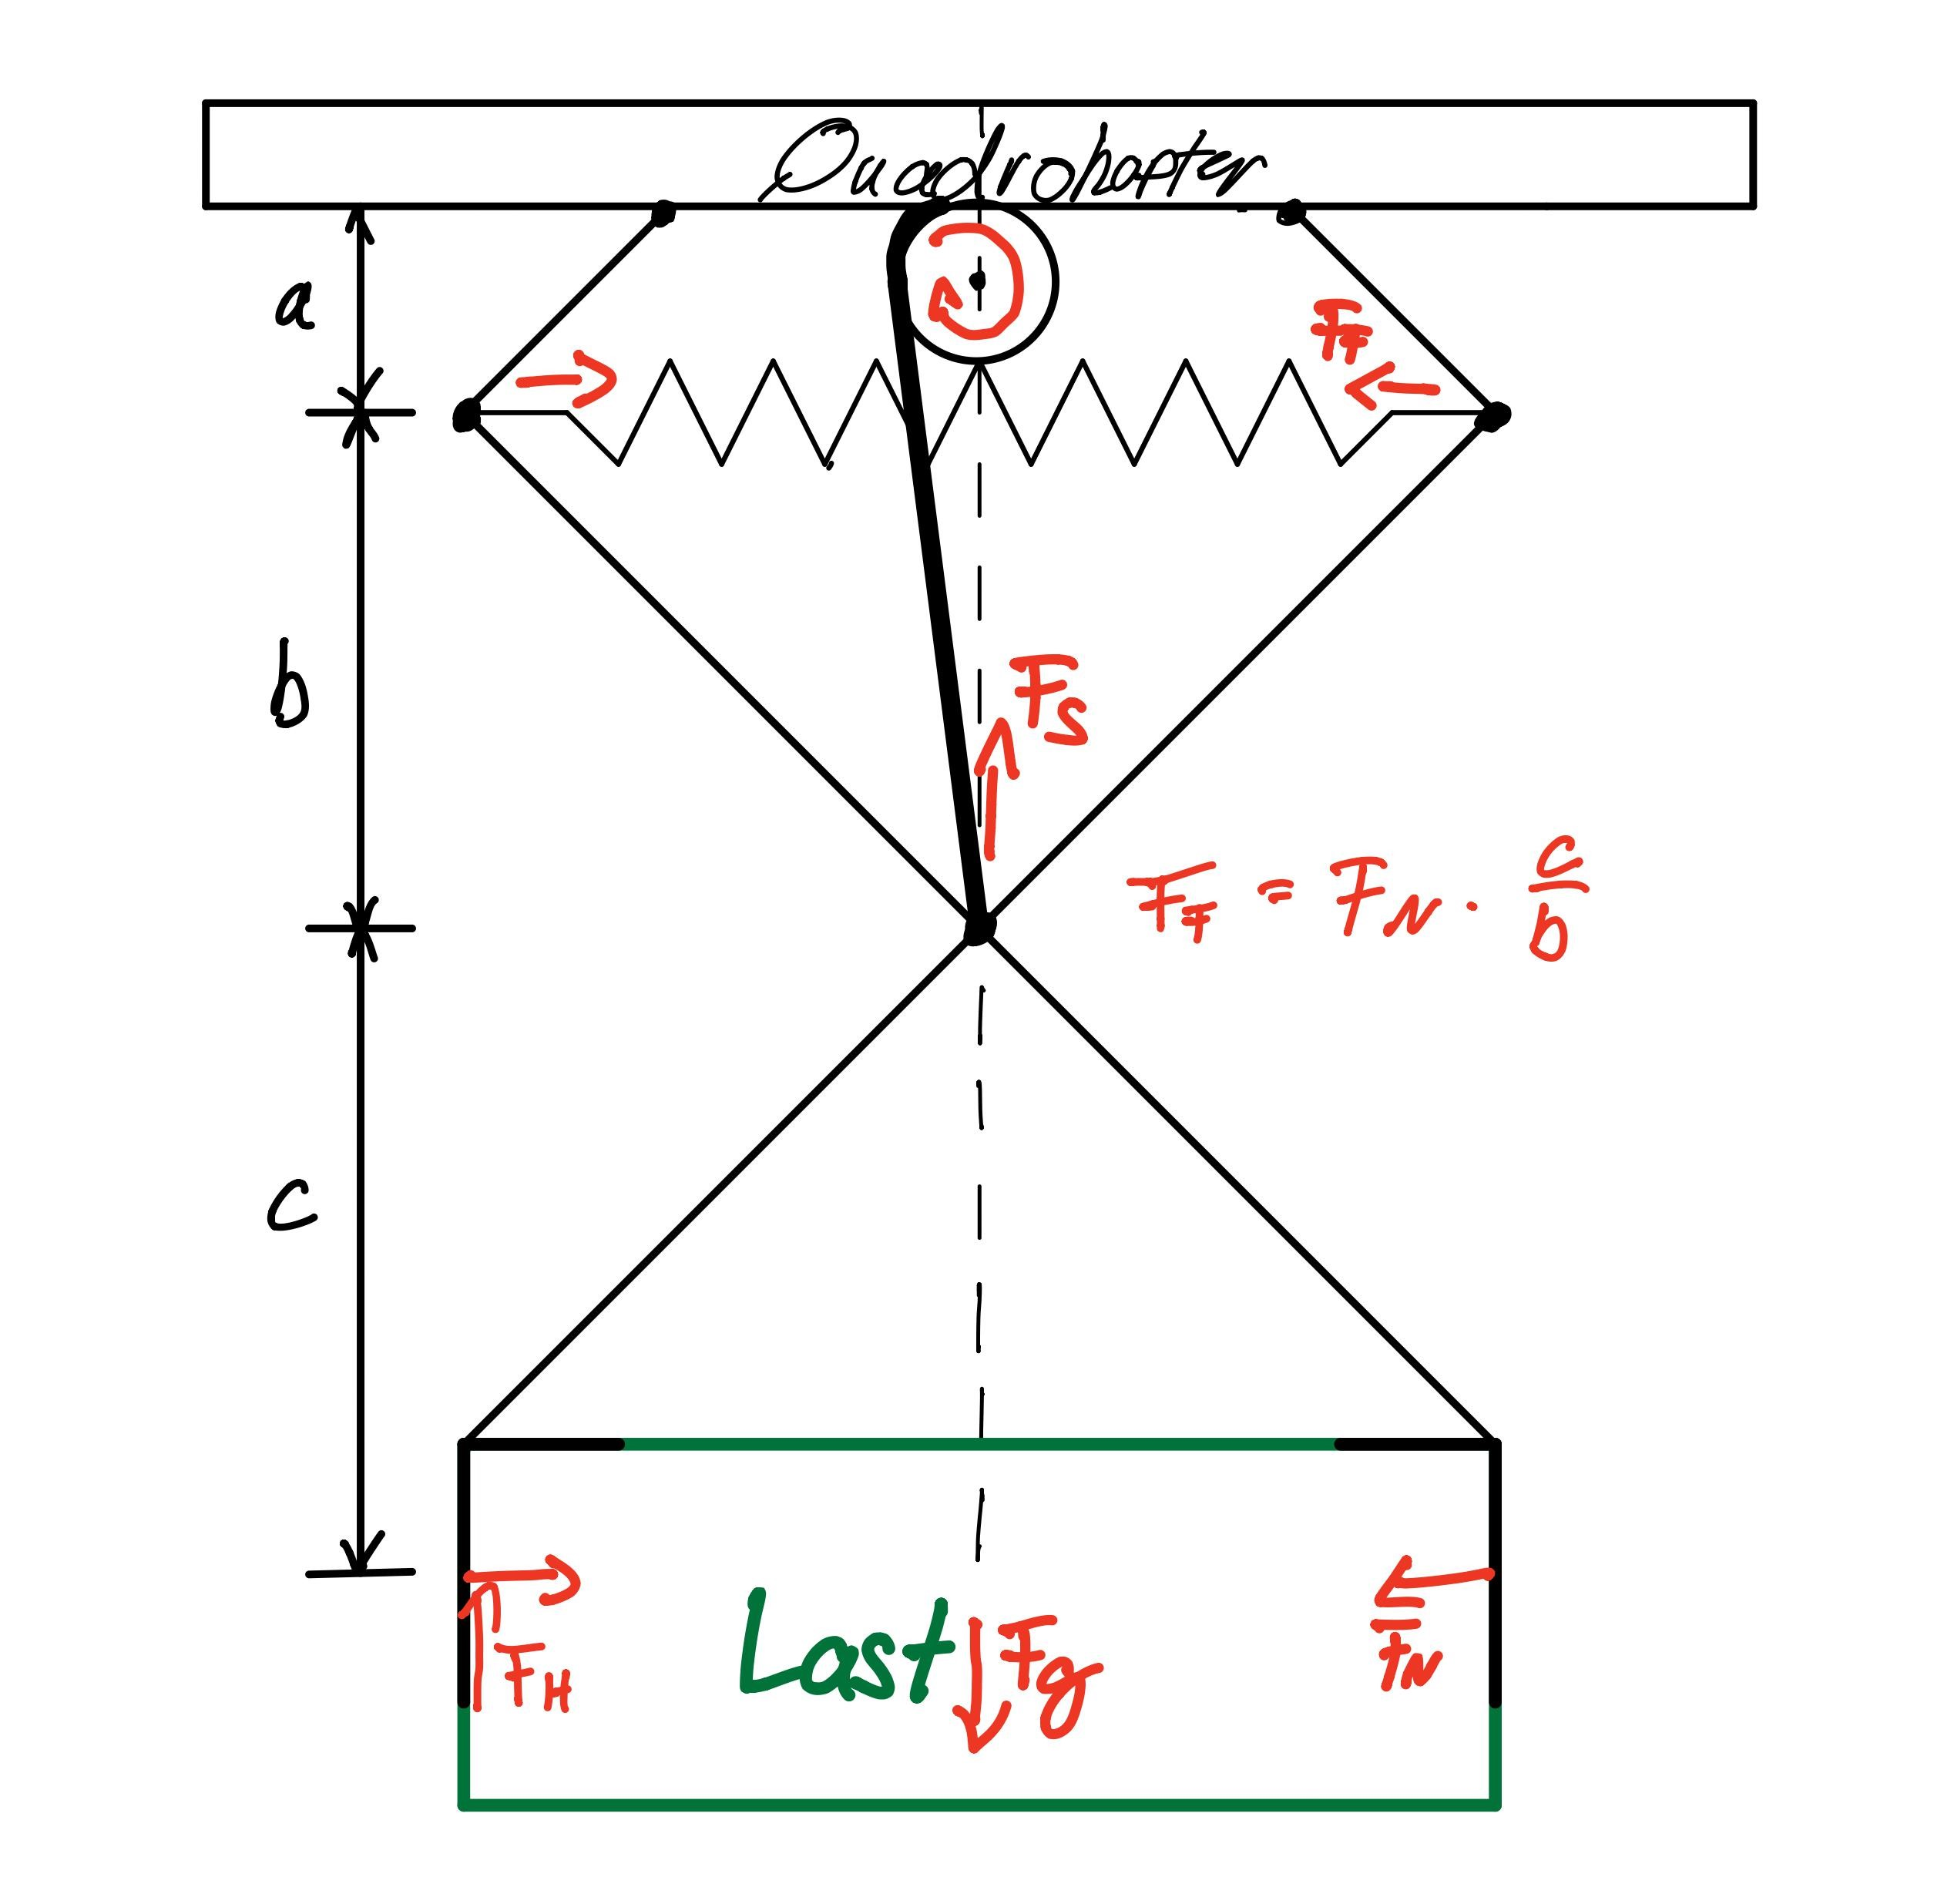
\includegraphics[scale=0.5]{Grafiken/Skizze1mechanik.jpg}
\caption{Erste Prinzipskizze}
\label{erste_prinzipskizze}
\end{center}
\end{figure}

\subsubsection{Vorteile:}
-	Relativ simpler Aufbau
-	Geringer Bauraum benötigt
-	Greifarm bleibt auch bei technischen Problemen durch die Federkraft geschlossen
-	Parallele Bauweise möglich, aber nicht notwendig (bringt Stabilität) 

\subsubsection{Nachteile:}
-	Ansteuern der Last erfordert durch Greifarme hohe Präzision
-	Rutschfestigkeit bei Greifarmen ungewiss
-	Federdimensionierung im kleinen Bauraum ungewiss
-	Sauberes Ab- und Aufrollen des Seils ungewiss
-	Lebensdauer der Feder mit leichtem Werkstoff ungewiss (Haftkraft)

\subsection{2.Konzept}
Bei der Funktionsweise des zweiten Konzepts übernimmt ein elektrischer Hubzylinder die Arbeit. Dieser öffnet und schließt Greifarme und hält diese in Position mit seiner eigenen Steifigkeit.

\begin{figure}
\begin{center}
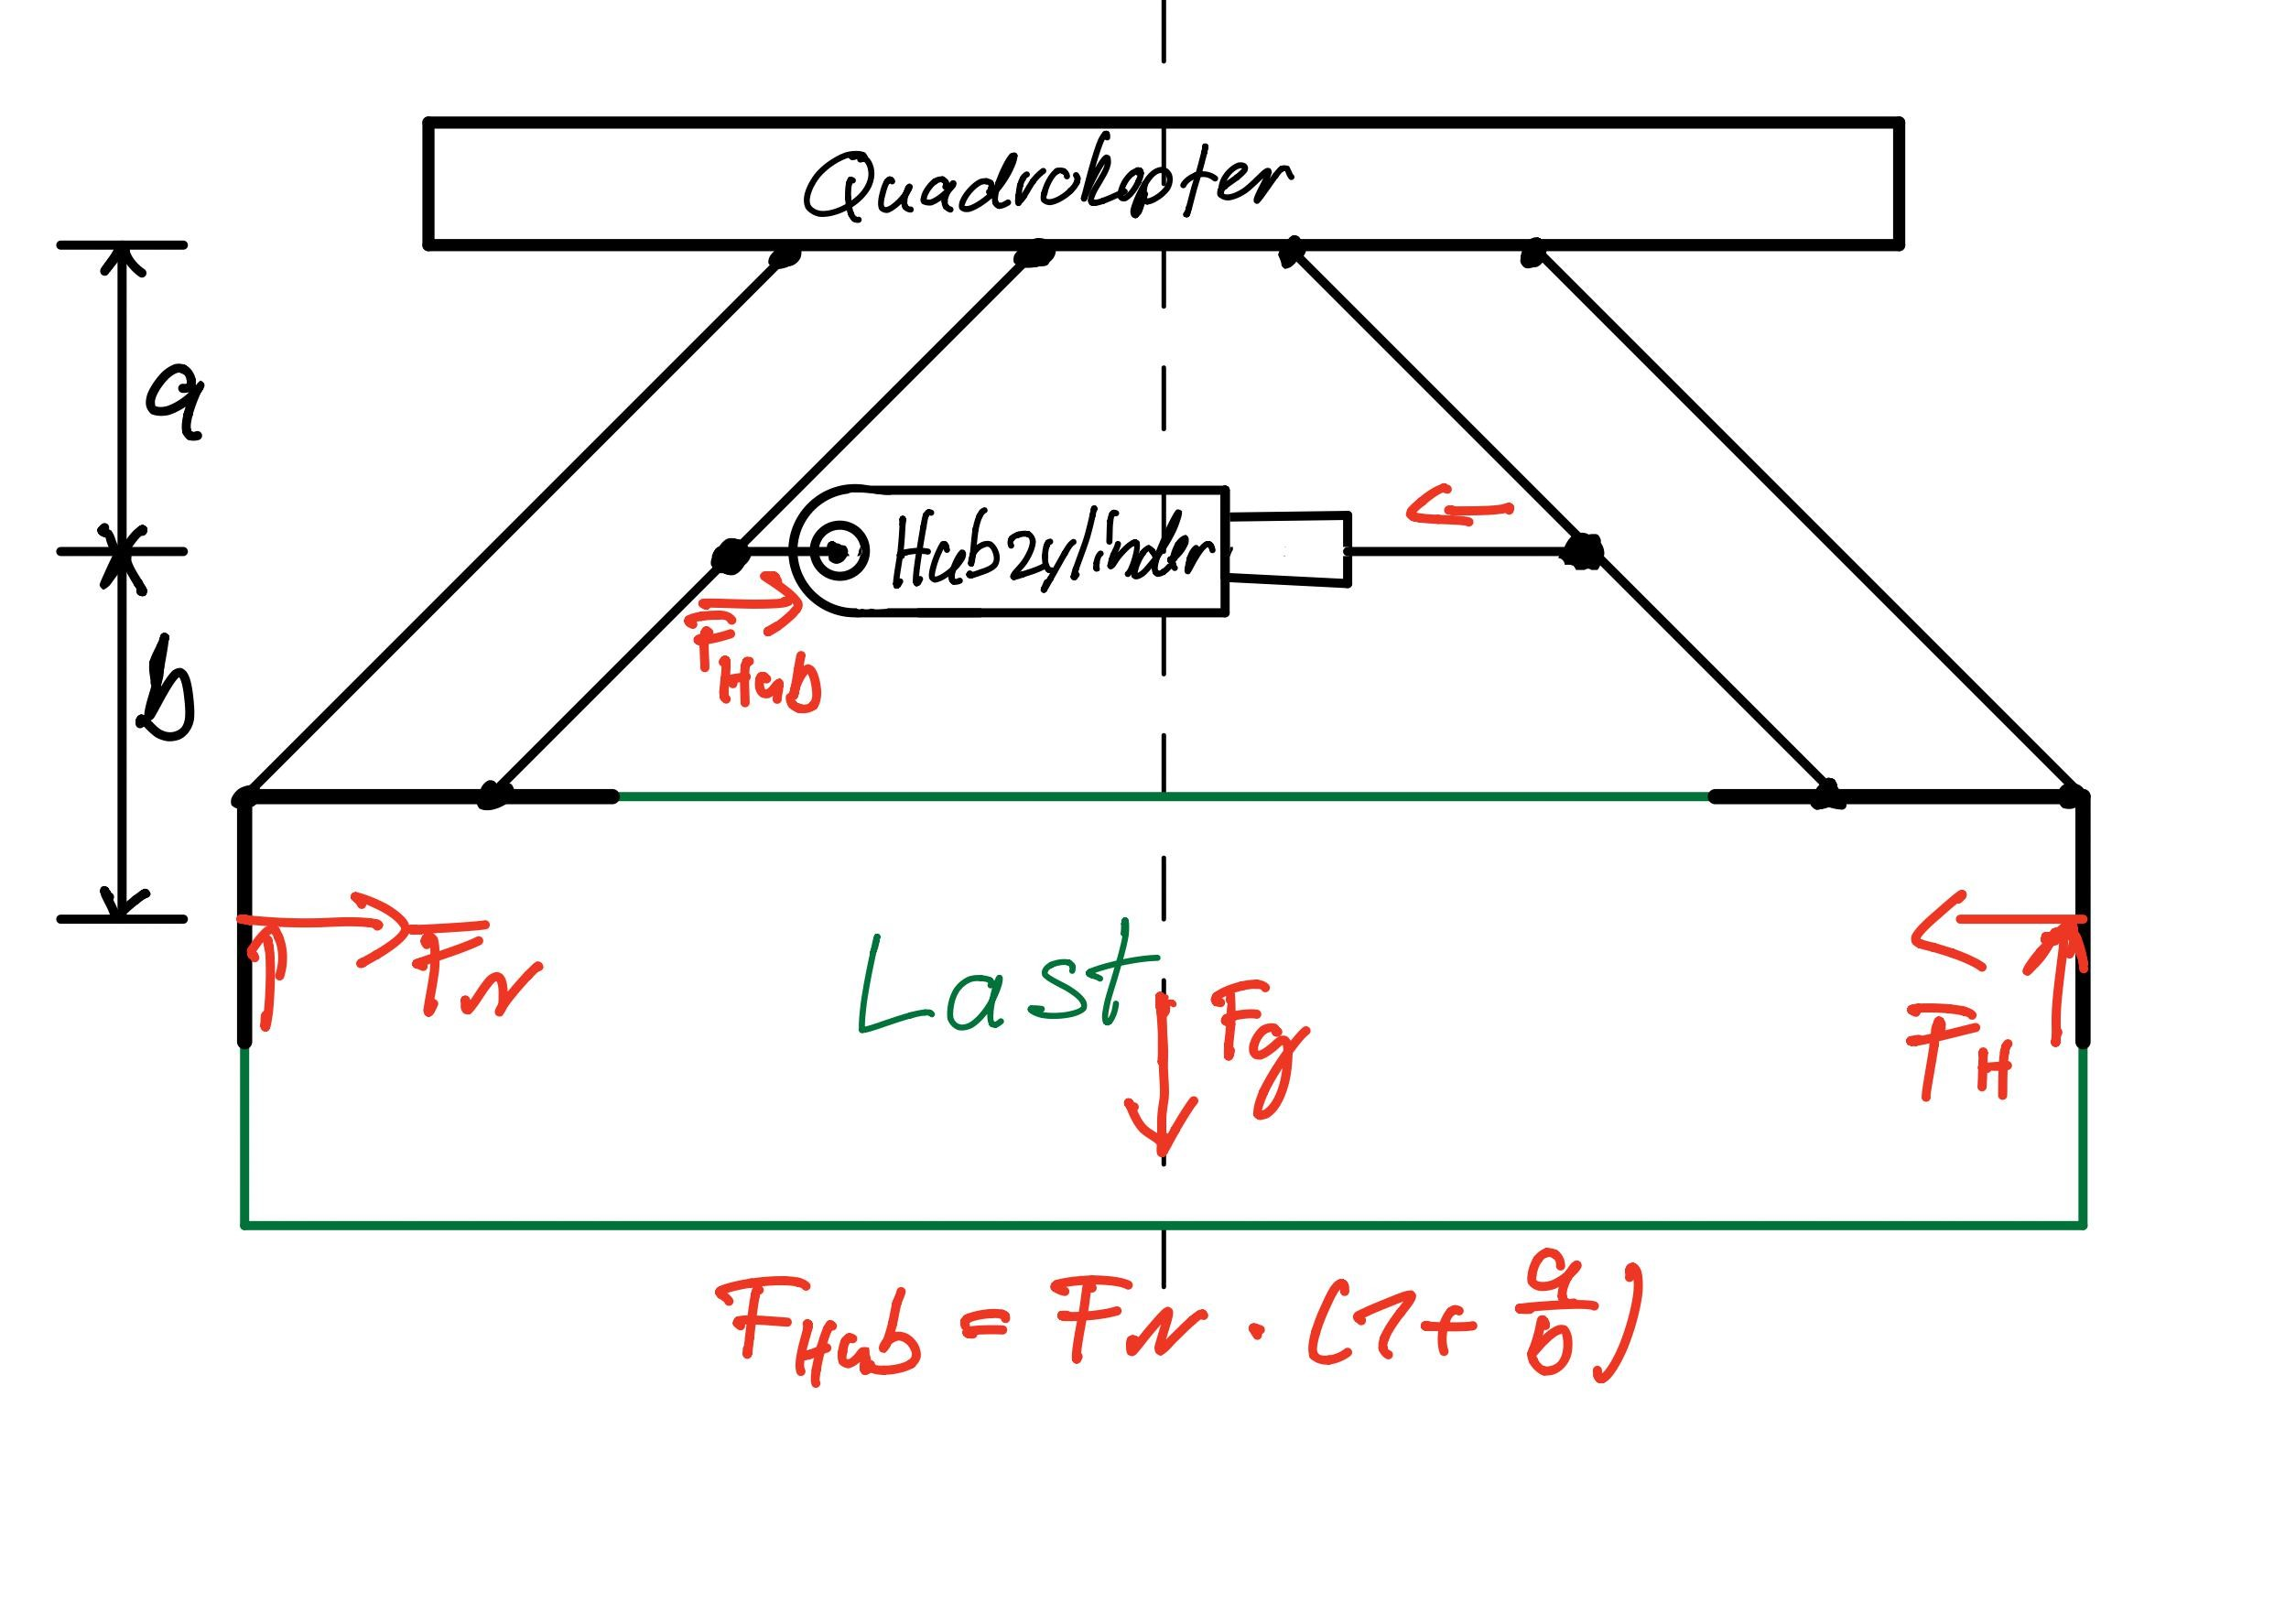
\includegraphics[scale=0.5]{Grafiken/Skizze2mechanik.jpg}
\caption{Zweite Prinzipskizze}
\label{zweite_prinzipskizze}
\end{center}
\end{figure}

\subsubsection{Vorteile:}
-	Simples Grundprinzip
-	Hubzylinder bleibt in Position (anders als bei einer Feder)
-	Parallele Bauweise bringt Stabilität
-	Präzises Ein- und Ausfahren der Greifarme für verschiedene Paketgrößen möglich 
-	Kameraposition kann zentriert werden im Zwischenraum

\subsubsection{Nachteile:}
-	Ansteuern der Last erfordert durch Greifarme hohe Präzision
-	Rutschfestigkeit bei Greifarmen ungewiss
-	Großer Bauraum nötig durch Parallele Bauweise und horizontalen Hubzylinder

\subsection{3.Konzept}
Hinter der Funktionsweise des dritten und letzten Konzepts verbirgt sich ein Knickgelenk an dessen Ende ein Magnet ist. Dieses Knickgelenk wird mittels zwei Motoren ausgefahren.

\begin{figure}
\begin{center}
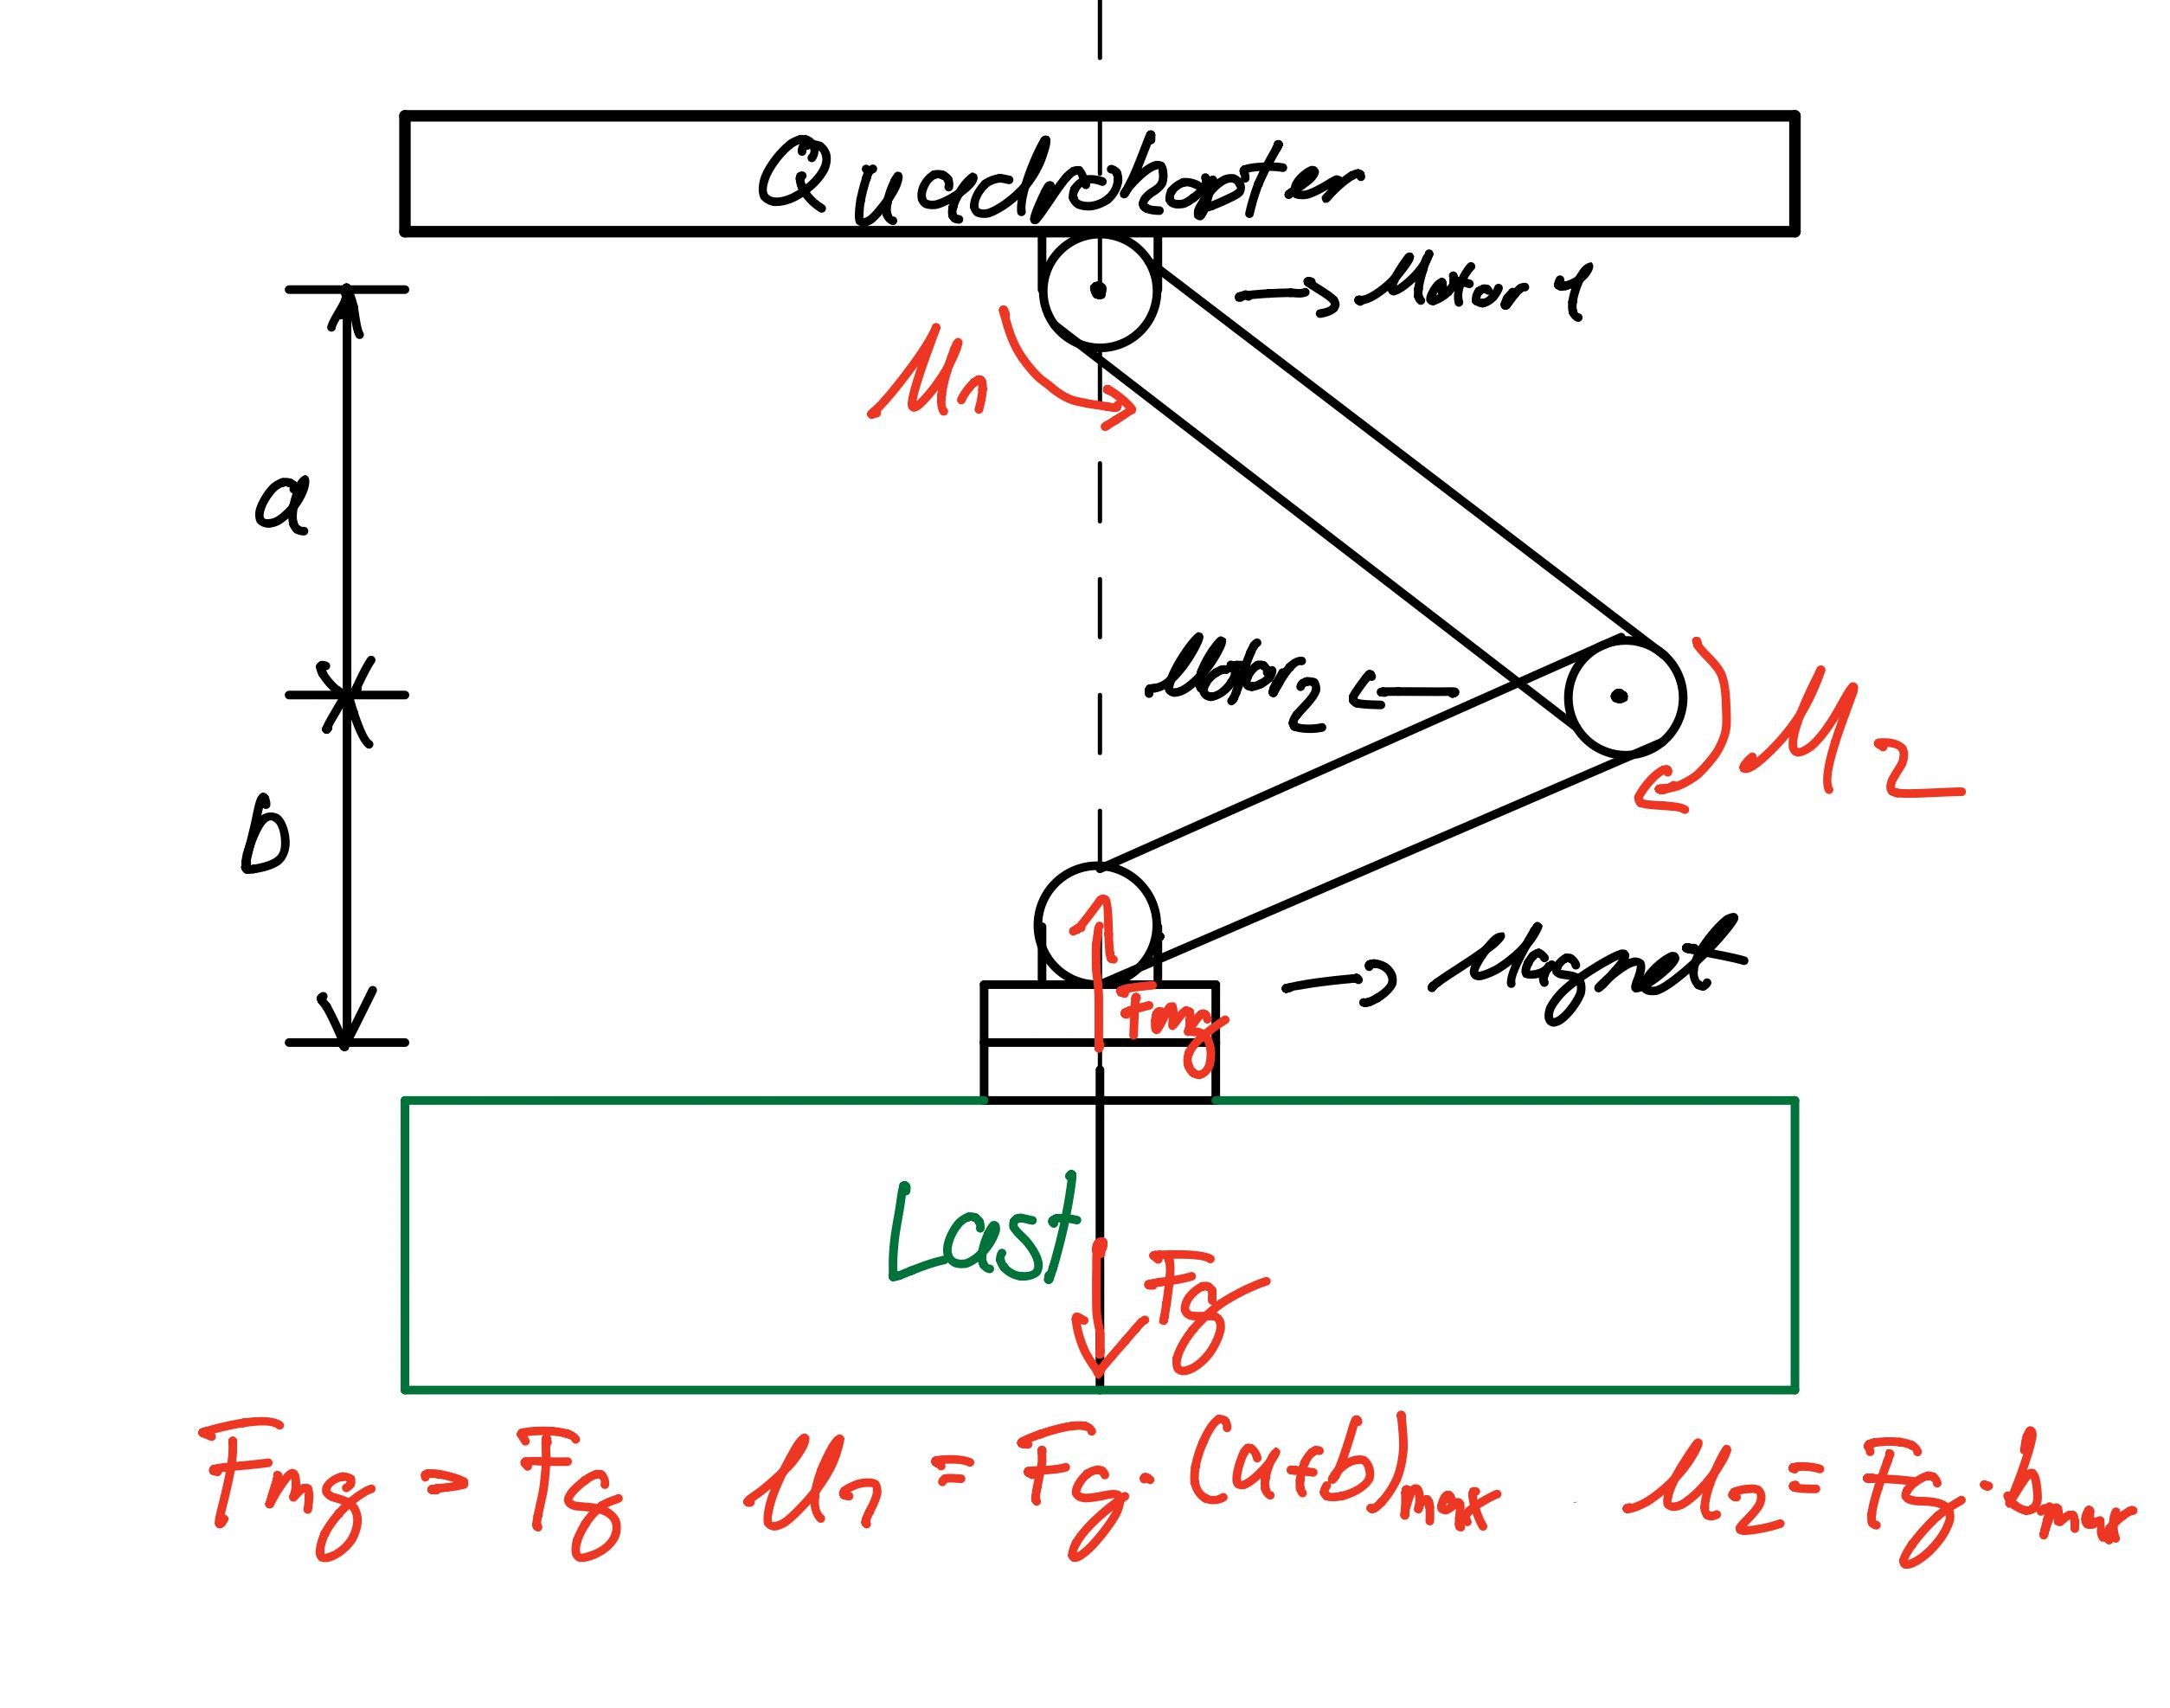
\includegraphics[scale=0.5]{Grafiken/Skizze3mechanik.jpg}
\caption{Dritte Prinzipskizze}
\label{dritte_prinzipskizze}
\end{center}
\end{figure}

\subsubsection{Vorteile:}
-	Kein richtiger „Greifarm“, weshalb es nicht mehr unbedingt auf die Reibung ankommt
-	Einfaches Ansteuern der Last beim Beladen
-	Schwerpunkt kann sehr gut mittig gehalten werden

\subsubsection{Nachteile:}
-	Gewichts erhöht durch zwei angebaute Motoren
-	Kameraposition ist nicht gutzentrierbar 
-	Erhöhte Komplexität durch zweiten Motor

\subsection{Konzeptauswahl}
Für ein letztendliches Fazit werden Vor- und Nachteile der vorgestellten Konzepte verglichen und abgewogen, um ein finales Konzept auszuwählen.
\
Dabei überzeugt das zweite Konzept am meisten, da der Hubzylinder einen stabilisierenden Faktor ins System mit einbringt und sich nur in der Länge verändert, wenn er das elektrische Signal dafür bekommt. Außerdem sind die simple Bauweise und gleichzeitig stabile Konstruktion weitere Faktoren, welche für das Konzept sprechen. Der Hauptfokus liegt demnach im Bauraum und der Länge des elektrischen Hubzylinders, wobei zweiteres als Zukaufteil nicht beliebig variabel ist. Ebenfalls ist die Leistung des Hubzylinders zu beachten, da er bei einem Material wie Plexiglas durchaus in der Lage ist, dieses, bei einem Fehler des Systems, zu zerstören.

\section{Berechnung und Vordimensionierung}
Bei der Berechnung und Vordimensionierung der Greifarmmechanik liegt der Hauptfokus auf dem Bauraum, dem Gewicht des Systems und der letztendlichen benötigten Kraft, welche von dem elektrischen Hubzylinder geleistet werden soll, um das Gewicht fest im Griff zu haben. Ersteres wird durch die Höhe und Lage der Standbeine des Quadrokopters begrenzt. Grobe Messungen ergaben einen Bauraum von $80 x 80 x 130 mm^3$. Dieser lässt sich jedoch durch genaue Formanpassung der Plexiglasteile in die Länge erweitern.

\subsection{Benötigte Normalkraft}

Die letztendlich wichtige Kraft ist die wirkende Hubzylinderkraft, welche in Form der Normalkraft an der Greiffläche wirkt. Letztere lässt sich mittels Reibgesetze berechnen. Da die Greifebene zum tragenden Objekt eben ist, ist die Greifebene zur Horizontalen senkrecht. Die Skizze verdeutlicht die Verteilung der Kräfte.

\begin{figure}
\begin{center}
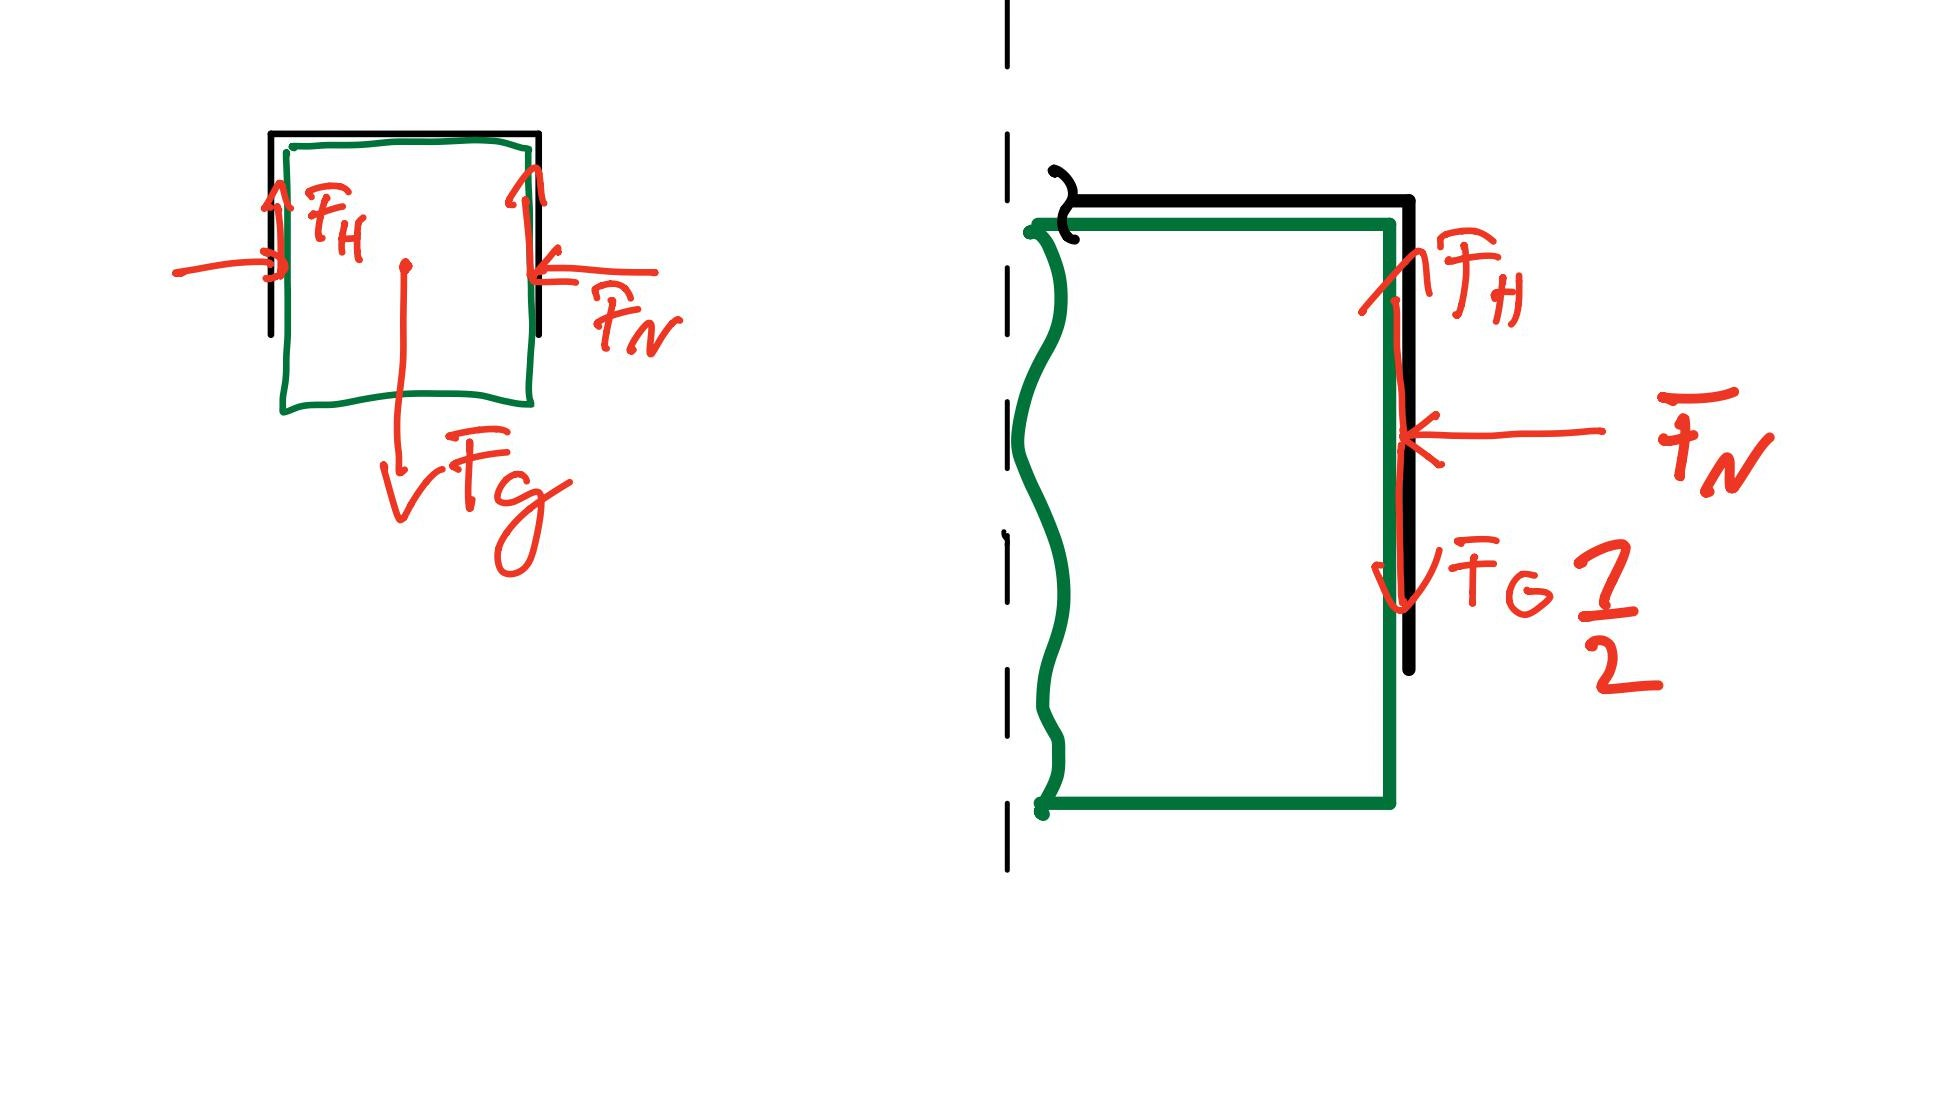
\includegraphics[scale=0.5]{Grafiken/Greiferflaeche.jpg}
\caption{Kraftverteilung an der Greiferfläche}
\label{greiferfläche}
\end{center}
\end{figure}

Aus der Skizze ergibt sich, dass die letztendlich benötigte Normalkraft abhängig von der Gewichtskraft und dem Haftreibwert ist. Da sich die Reibwerte zu jeweiligen Gleitebenen verschiedener Materialien nur experimentell erörtern lassen, muss ein Mittelwert genommen werden, welcher nach den ersten Experimenten eventuell zu korrigieren ist. Als Oberflächen werden Gummi und Plexiglas genommen. Nach längerer Recherche setzt sich ein ungefährer Mittelwert von $u_H = 0,3$ durch \cite{Haftreibungszahl}.

Für die zu ermittelnde Gewichtskraft ist von einem Gewicht von 50g bis 100 g für die Last zu schätzen. Um eine gute Fehlertoleranz und damit Sicherheit zu bieten, wird der errechnete Wert mit dem Faktor $S = 1,8$ angepasst.
Mit dem gegebenen Haftreibwert und der Erdbeschleunigung $g = 9,81 \frac{m}{s^2}$ auf die Last, lässt sich nun die nötige Haftkraft in Form der Normalkraft berechnen:

\begin{equation}
\frac{1}{2}*F_G = F_H
F_G = m*g
F_H = F_N*u_H
m*g = F_N*u_H*2
F_N = \frac{m*g}{u_h*2} = \frac{0,1kg*9,81*\frac{m}{s^2}}{2*0,3} = 1,635N
F_Nmin = F_N*S = 1,635N* 1,8 = 2,943N
\end{equation}

Aus der Rechnung ergibt sich also eine ungefähr benötigte Normalkraft von $F_Nmin = 3$.

\subsection{Benötigte Hubzylinderkraft}

Die schlussendlich benötigte Hubzylinderkraft lässt sich über einfache Hebelgesetze mit der Normalkraft schlussfolgern. Anhand der Skizze und den darauf rotierenden angedeuteten Hebelarmen, erkennt man, dass die maximale Hebellänge in senkrechter Stellung erreicht ist. Die Wahl des Hebelverhältnisses zwischen a und b ist hier entscheidend. Denn Bauraum und Maße der in Frage kommenden Hubzylinder setzen hier starke Grenzen. Für die grobe Vordimensionierung wird das Verhältnis von a zu b auf 1:1 gesetzt.

\begin{figure}
\begin{center}
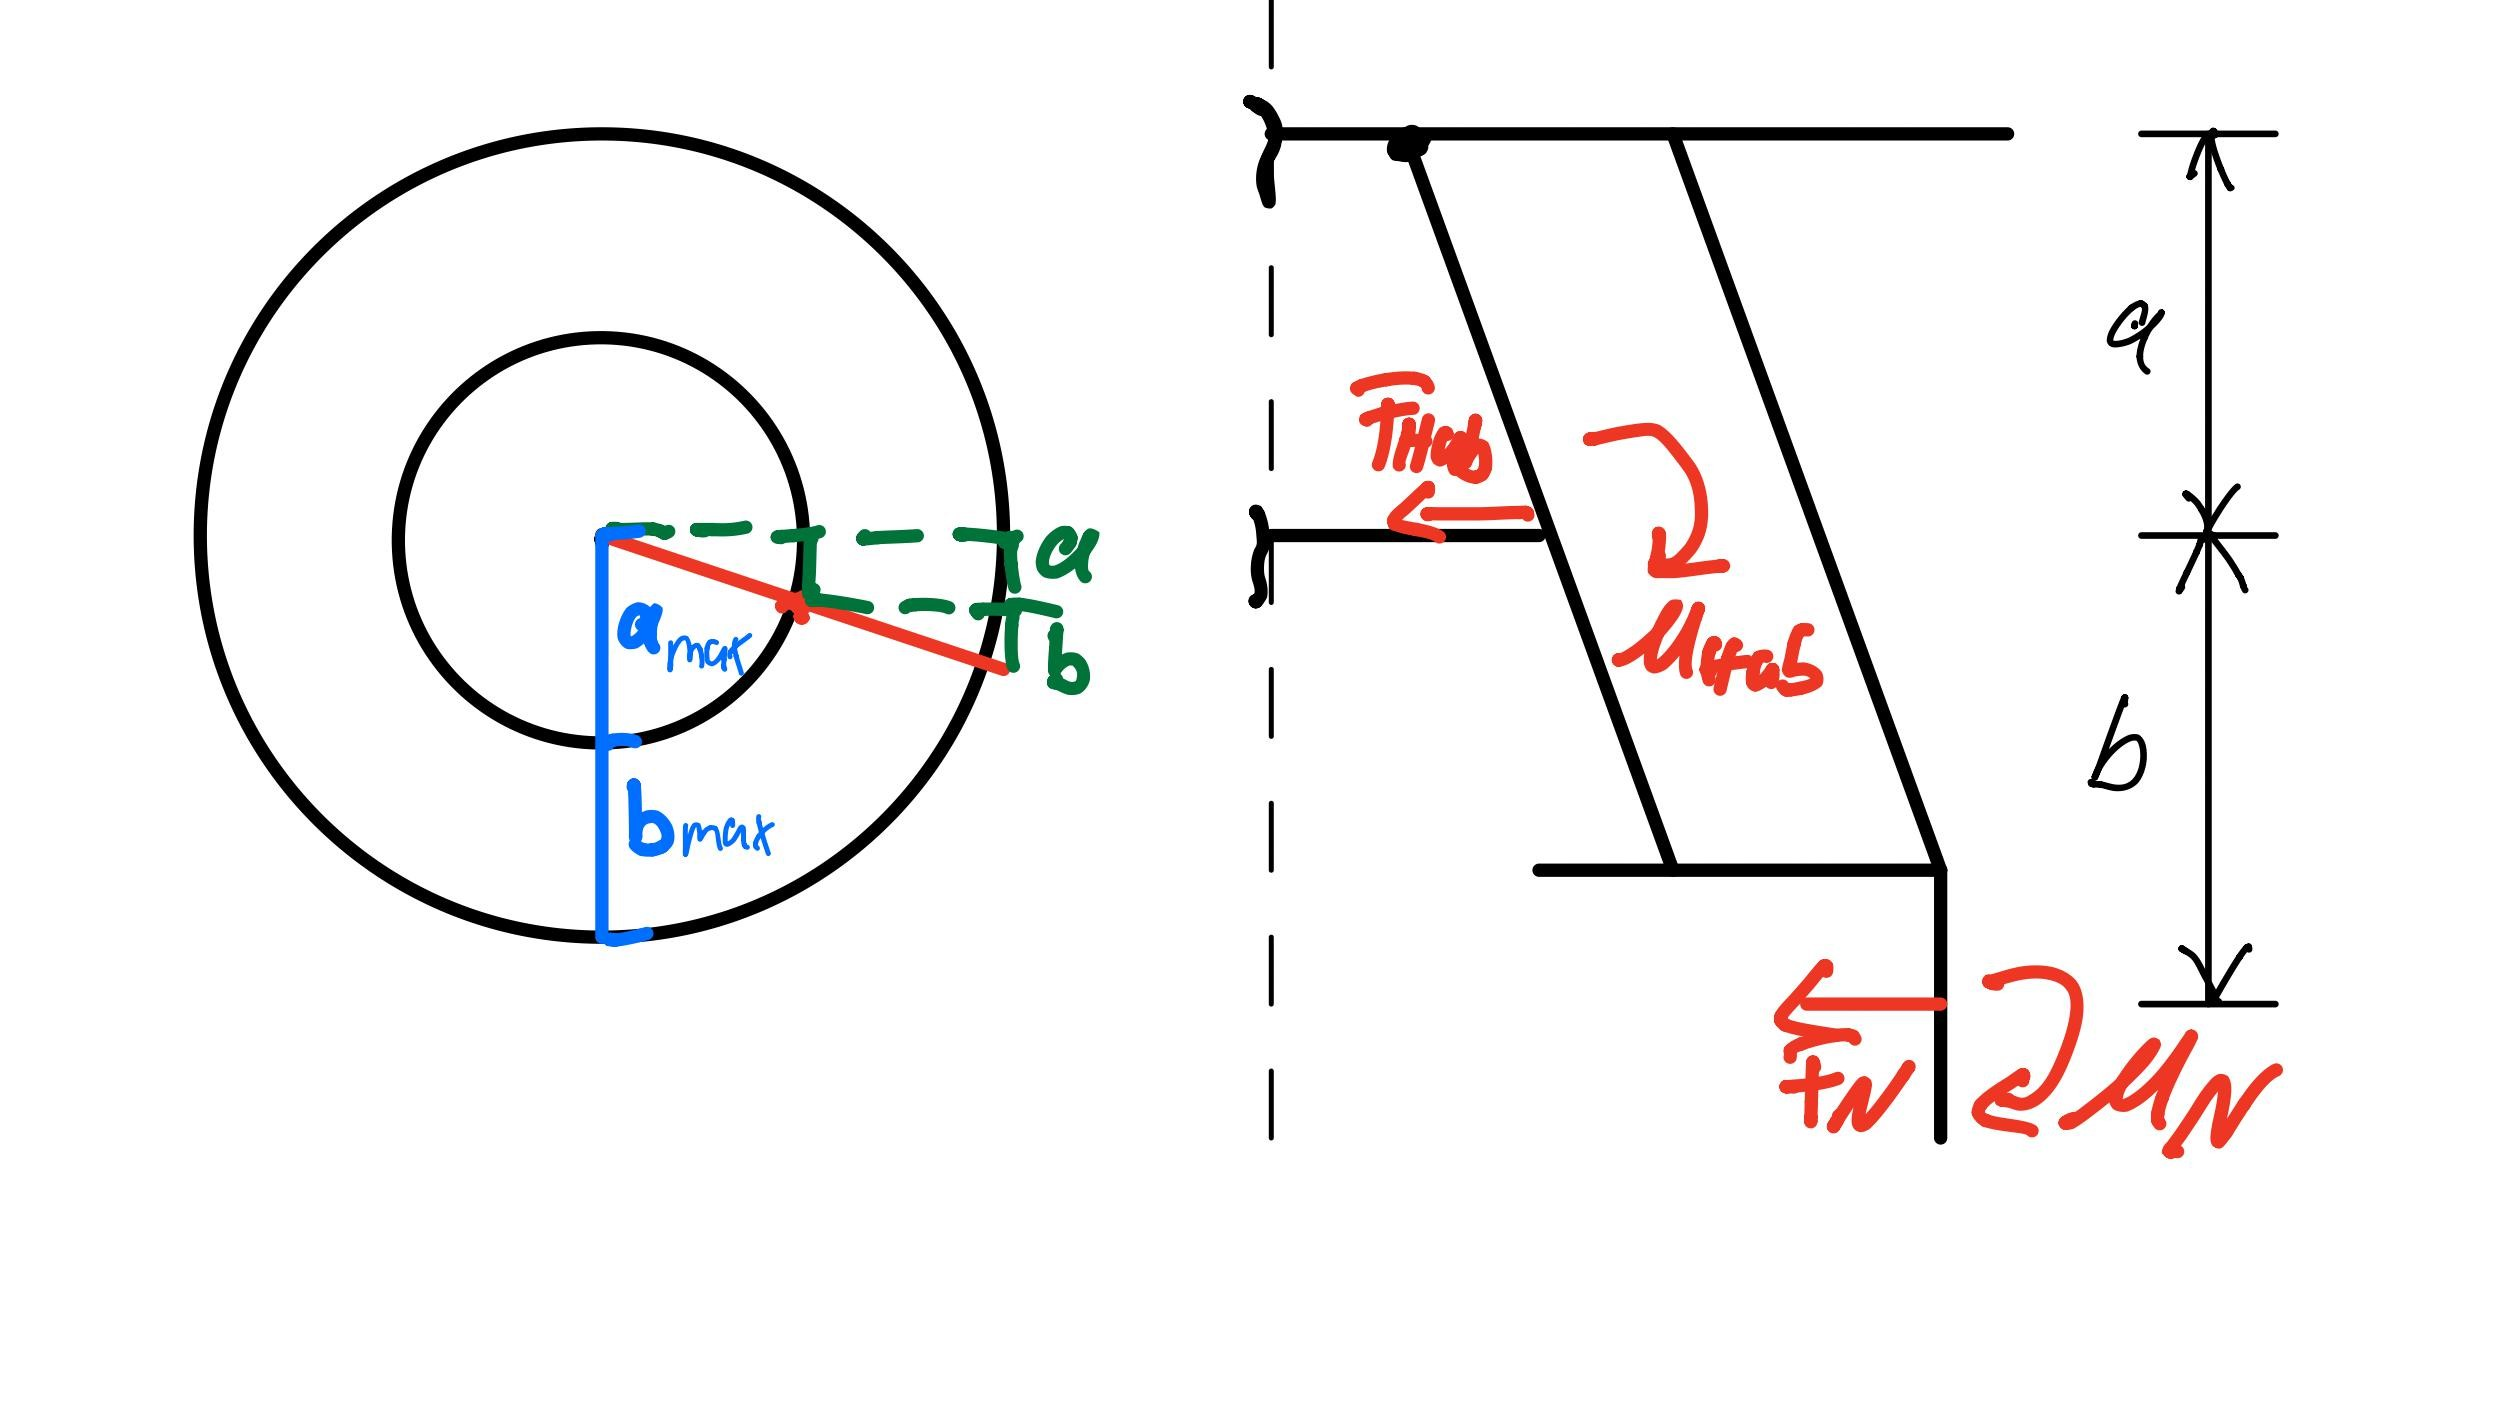
\includegraphics[scale=0.5]{Grafiken/Mechanikskizze.jpg}
\caption{Kraftverteilung an den Hebelarmen}
\label{mechanikskizze}
\end{center}
\end{figure}

\begin{equation}
F_N*(a + b) = F_Hub*a
F_Hub = F_N*(1 + \frac{b}{a}) = F_N*2 = 6N
\end{equation}

\subsection{Auswahl des Hubzylinders}
Mit der berechneten Hubzylinderkraft von $6N$ fällt die Wahl des elektrischen Hubzylinders auf den „Titan 30“ von CTI-Modellbau \cite{Titanzylinder}, welcher mit dem „Thor4HF Titan 1 Regler“, ebenfalls von CTI-Modellbau \cite{Titanregler}, betrieben wird. Durch den begrenzten Bauraum bieten sich nicht viele Alternativen an, da die Firma CTI-Modellbau sich explizit auf den Modellbau konzentriert.
Mit einer erwünschten Öffnungsbreite von jeweils 30 mm pro Seite und einem Faktor von 2, durch die mittige Position des Hubzylinders, lässt sich eine erwünschte Hublänge von 30 mm errechnen.

\section{Vom Modell zu den ersten Bauteilen}
\subsection{Creo Modell}
Mit den ersten vordimensionierten Bauteilen und den ersten festen Maßen von den Zukaufteilen, lässt sich nun ein erstes CAD-Modell bauen. Dabei werden je nach Absprache und Änderungen von Eigenschaften Anpassungen unternommen, um dem finalen Produkt so nah wie möglich zu ähneln. Aus dem CAD Modell, modelliert mit Creo Parametrics5, lässt sich schon die grobe Gestalt der Greifarmmechanik erkennen.

\begin{figure}
\begin{center}
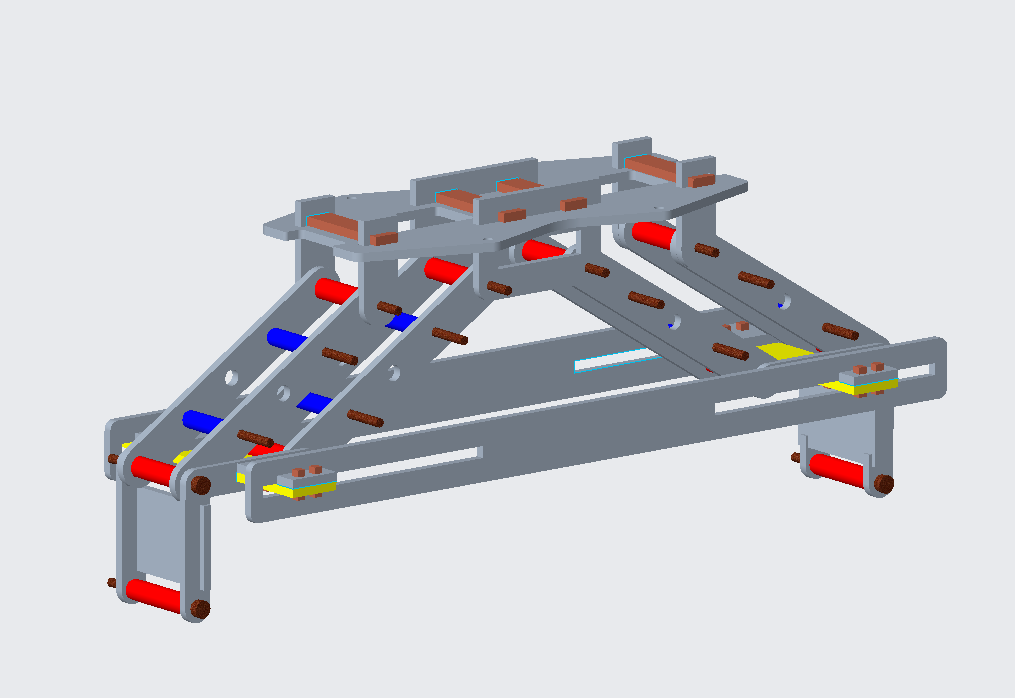
\includegraphics[scale=0.5]{Grafiken/Creo1.png}
\caption{Erstes CAD-Modelle}
\label{creo1}
\end{center}
\end{figure}

\subsection{Inkscape}
Die letztendlich fertigen CAD-Bauteile können nun mit „Inkscape“, eine Software zur Bearbeitung und Erstellung zweidimensionaler Vektorgrafiken, zu Schnittmustern erzeugt werden. Mithilfe dieser Schnittmuster werden die fertigen Bauteile aus den Plexiglasplatten von der Laserschneidemaschine ausgeschnitten.

\begin{figure}
\begin{center}
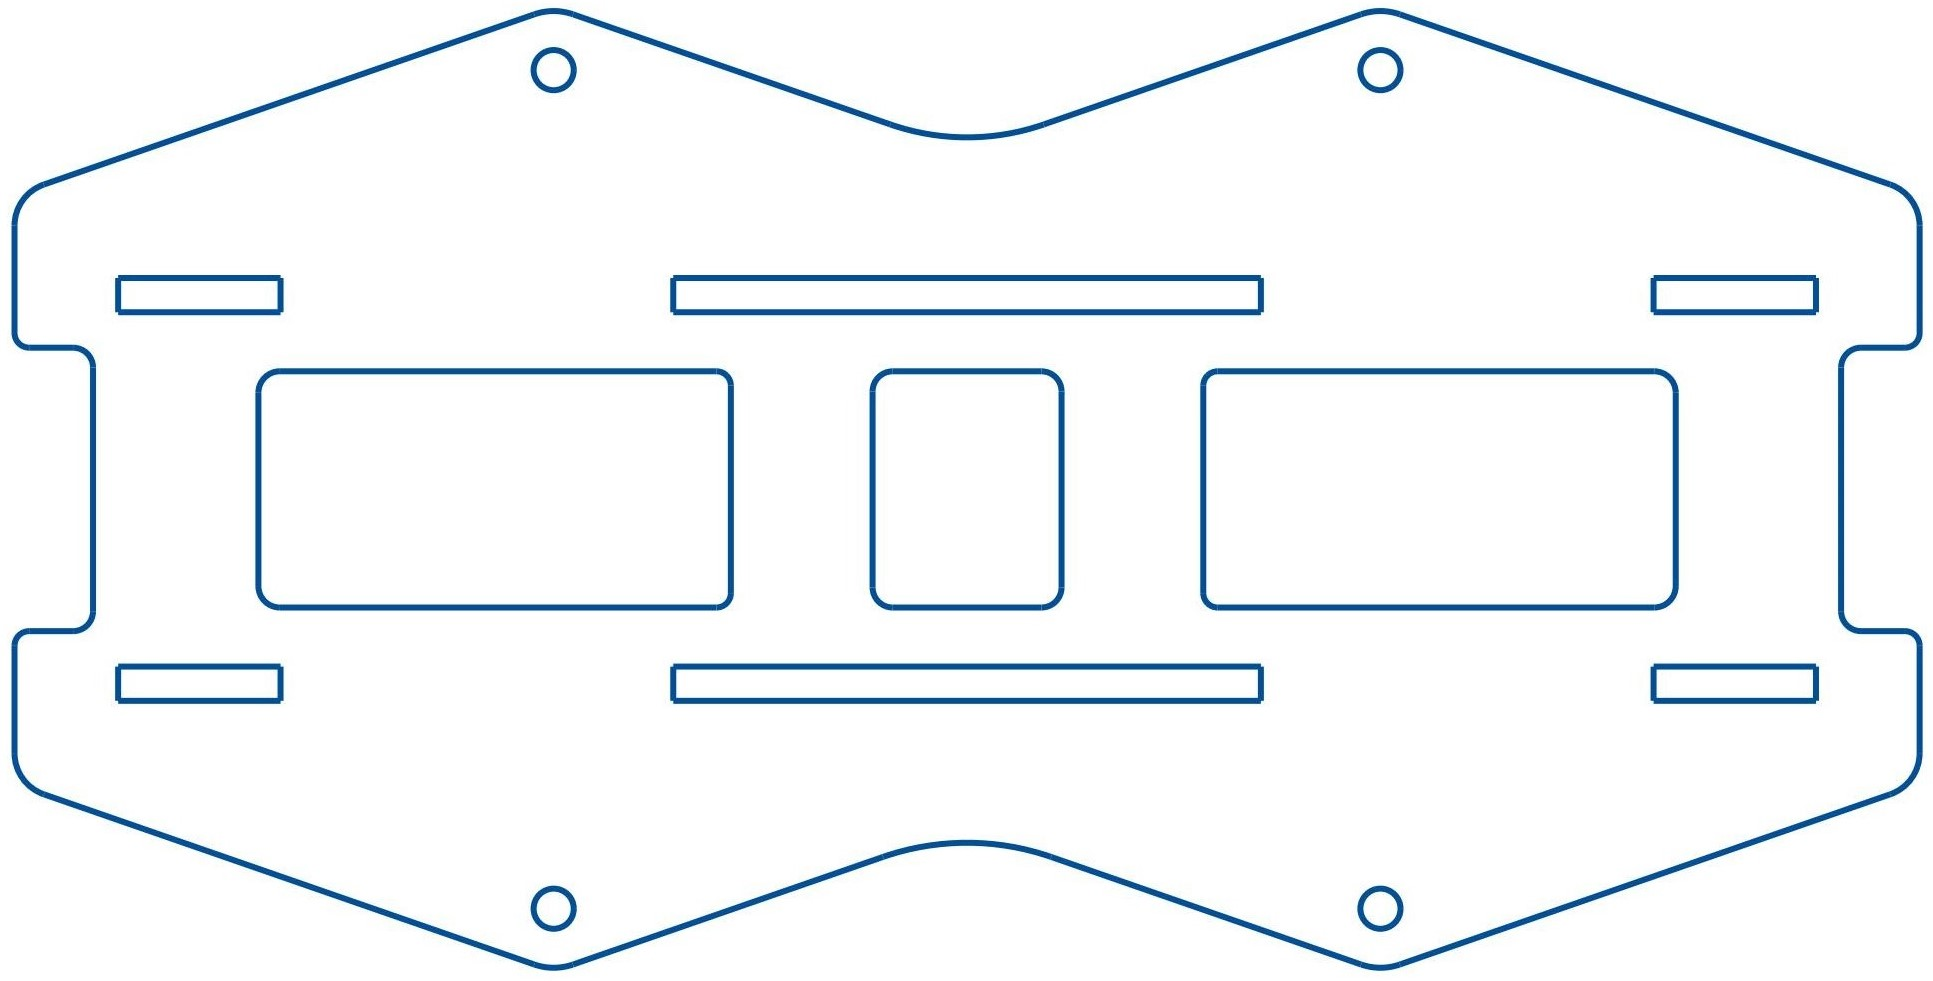
\includegraphics[scale=0.5]{Grafiken/Inkscapebodenplatte.jpg}
\caption{Inkscapeschnittmuster der neuen Bodenplatte}
\label{inkscape1}
\end{center}
\end{figure}

\subsection{Erste Ergebnisse}
Die ausgeschnittenen Bauteile werden zur Probe vormontiert, um mógliche Problemstellen ausfindig zu machen.

\begin{figure}
\begin{center}
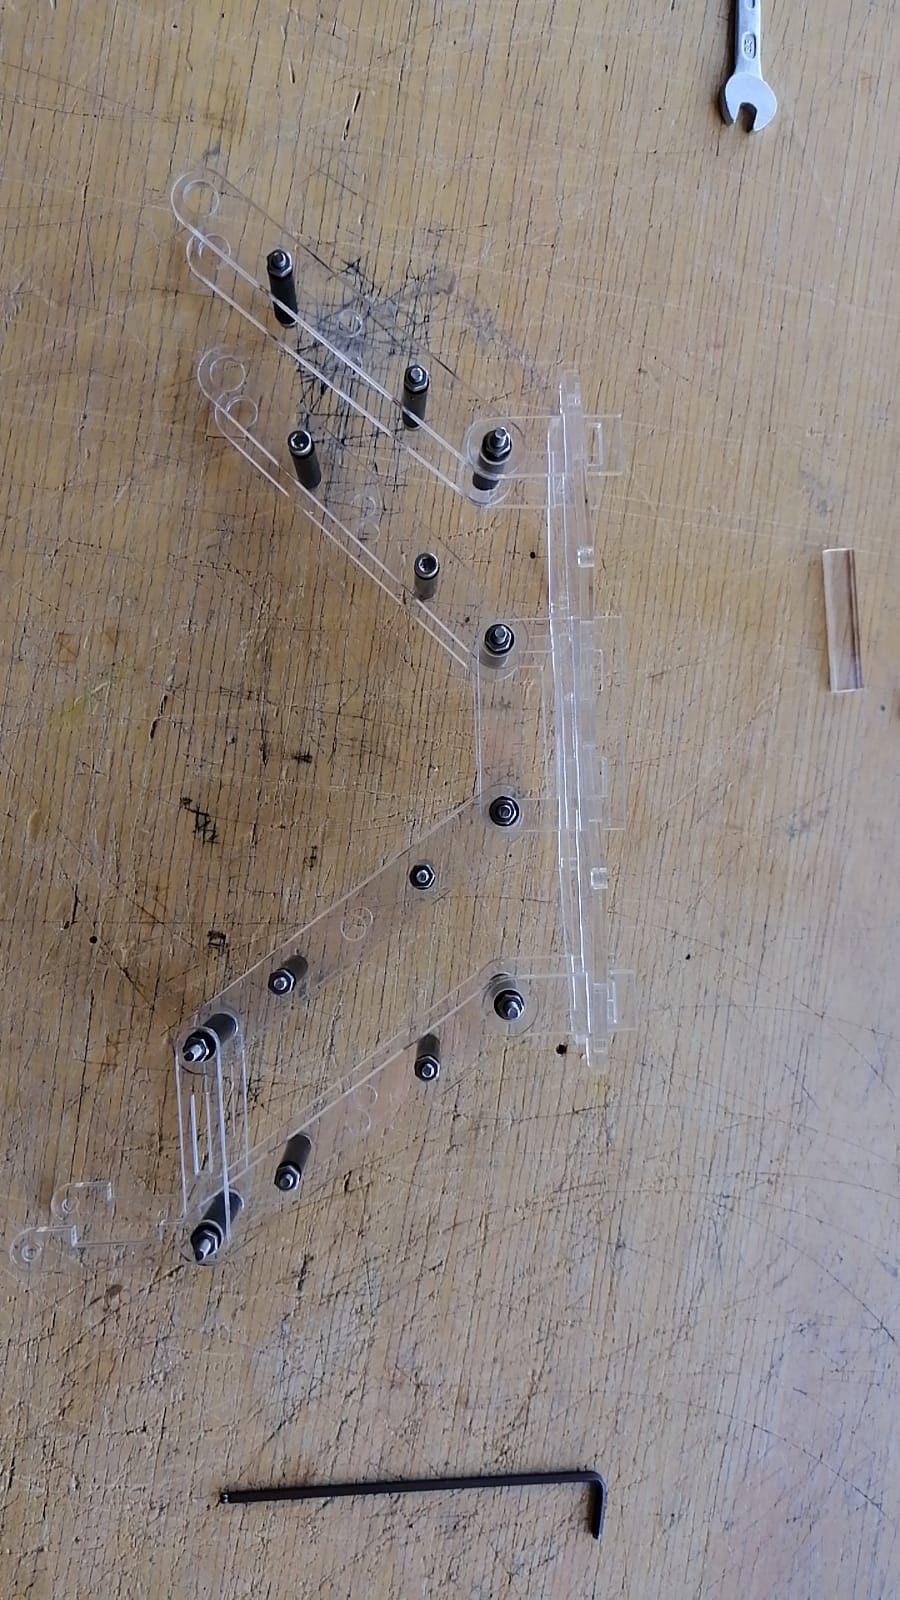
\includegraphics[scale=0.4]{Grafiken/Fotohebelarme.jpg}
\caption{Zusammengebaute Hebelarme}
\label{hebelarme}
\end{center}
\end{figure}

\begin{figure}
\begin{center}
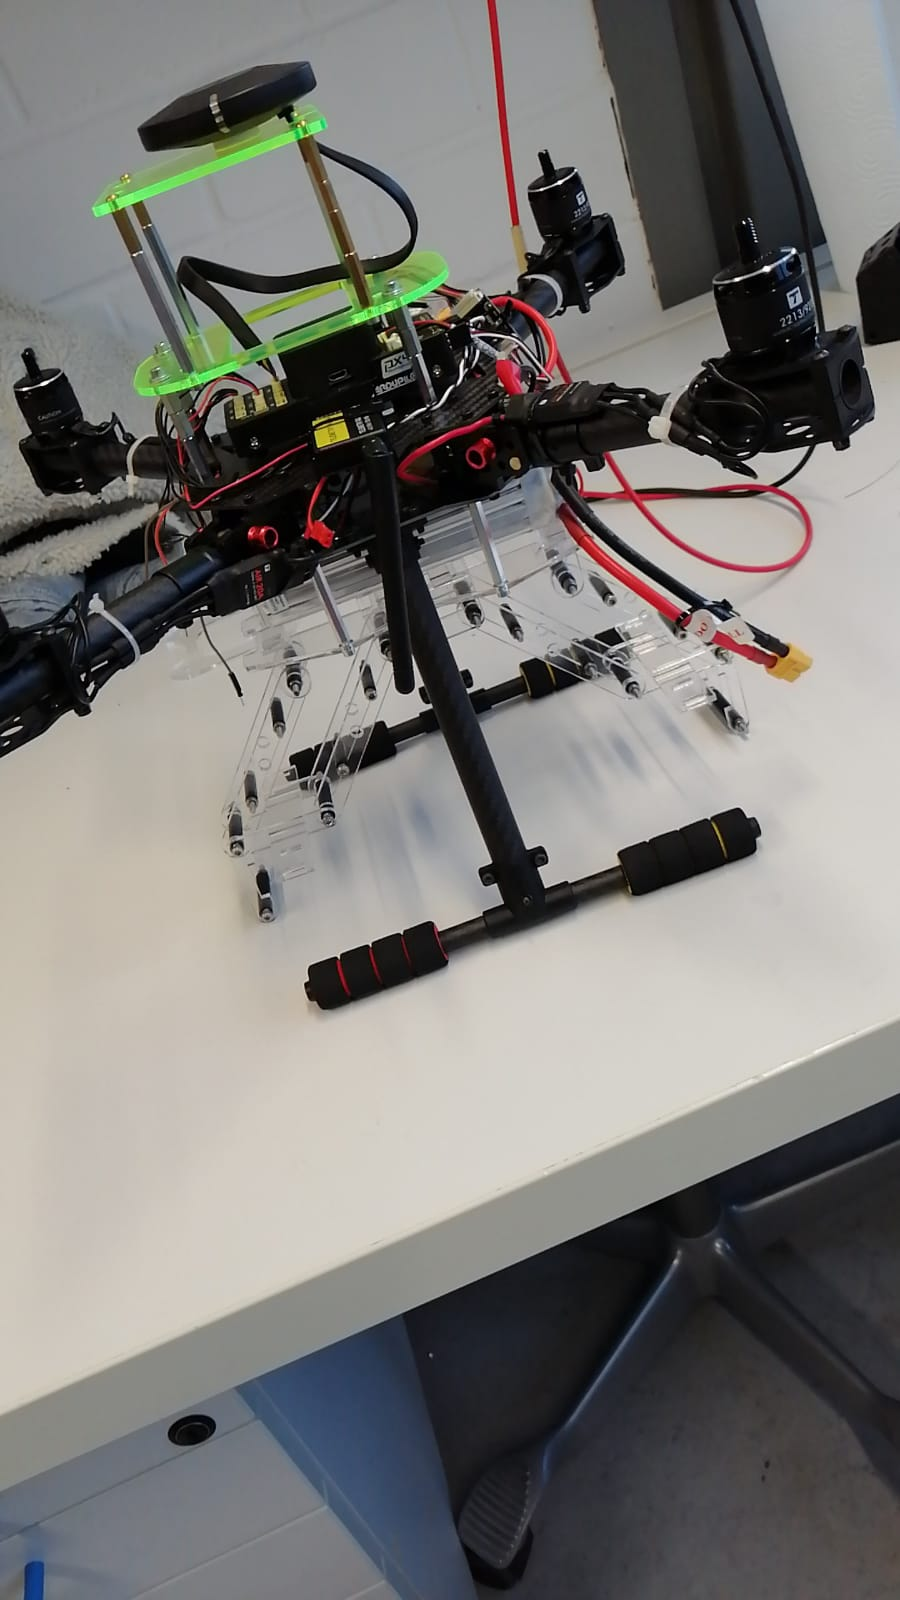
\includegraphics[scale=0.4]{Grafiken/Fotoquadrokopter.jpg}
\caption{Vormontage der Greifarmmechanik am Quadrokopter}
\label{vormontage}
\end{center}
\end{figure}

Um die aus den Berechnungen gewünschte Reibung zu erlangen wird auf den Flächen der Greifer noch eine Gummischicht draufgeklebt.
Nach der letztendlich fertigen Konstruktion muss für die Sensoren noch eine Befestigung hinzugefügt werden. Diese ist aber letztendlich stark vom eingenommenen Volumen des Greifsystems im Bauraum abhängig, da sie bestenfalls zentriert liegt und wird erst nach den ersten Testläufen beigefügt

\section{Problematiken und Lösungen}
Bei den ersten Testläufen ist vermehrt aufgefallen, dass die Wandstärken mit dem CAD Modell schlecht einschätzbar sind und demnach lange und dünne Bauteile so umkonstruiert werden müssen, damit die gewollte Steifigkeit von dem benutzten Plexiglas trotzdem noch erhalten bleibt.
\
Gleichzeitig muss auf die Anziehkraft der Schrauben geachtet werden, da bei zu hohen Kräften das Plexiglas durchbrechen könnte oder auch zu hohen Reibungskräften unterliegen würde, welche das System zu sehr unkontrolliert beeinflussen würde. Demnach sind alle Schrauben nicht komplett versteift eingeschraubt, was gleichzeitig zur Folge hat, dass Steifigkeit und Stabilität des Systems in gewissen Maßen drunter leiden. 
\
Auch funktioniert die Führungsschiene nicht so wie angedacht, da zu hohe Reibungskräfte zwischen den einzelnen Plexiglasflächen entstehen. Ein kurzer Umbau lässt nun die Führungsschiene das System, über die schon angebrachten Bolzen, an den Greifern führen. Auch diese Lösung ist nicht perfekt, denn wenn die Querkräfte zu hoch werden, verbiegt sich das Plexiglas und erfüllt demnach nicht mehr seine Funktion einwandfrei. Auch das ist mit einer erhöhten Wandstärke auf Kosten höheren Gewichts teilweise besser geworden. Da aber auch hier die Reibung zwischen Führungsbolzen und Plexiglas nicht komplett zu verhindern ist, lässt sich das Problem nicht ganz lösen.
\
Ein weiteres Problem ist der Öffnungswinkel des Systems. Denn um 60 mm gewollten Öffnungsspalt zu erreichen, müssten die Hebel weiter voneinander entfernt liegen, was das Volumen des Greifarms noch größer machen würde. Denn die Länge des Hubzylinders ist nicht stark variabel, weshalb der Bauraum zur Mitte hin begrenzt ist. Der momentane Öffnungsspalt von 45 mm sollte demnach erstmal beibehalten werden, da Verbesserungen größere Maßnahmen erfordern würden.

\section{Fazit zur Mechanik}

Bei der letztendlichen Fertigstellung der Mechanik zeigt sich die Komplexität darin die Balance zwischen Leichtbau, Stabilität und Steifigkeit beizubehalten, ohne dabei die Funktion des Greifarms einzuschränken und das mit einfachsten Mitteln. Der Verzicht auf einen Elektromagneten für die Greiffunktion führt zu einem großen eingenommenen Bauraum und viel Zusatzgewicht, da die Konstruktion der Greifarme für die anliegenden Kräfte eine gewisse Stabilität brauchen. In realitätsnahen Szenarien werden Faktoren wie zuverlässige Stabilität und möglichst lange Akkulaufzeiten jedoch benötigt. Dies stellt sich als eine zukünftige Hürde für andere Projekte dieser Art heraus. Die Grundfunktion an sich wird jedoch erfüllt.
\
Das Bauen ohne zuverlässige Lagerung erwies sich auch nicht als einfach und kostete dem System weitere Stabilität. Auch der enorme Bauraum, generiert durch den Hubzylinder, setzt dem System starke Grenzen und führt zu einem erhöhten Gewicht.
